\lstset{basicstyle=\ttfamily,
	showstringspaces=false,
	commentstyle=\color{red},
	keywordstyle=\color{blue},
	frame=single
}

\capitulo{4}{Técnicas y herramientas}


\section{Técnicas}
En esta sección se explicarán las distintas técnicas utilizadas a lo largo del proyecto.

\subsection{Scrum}
Scrum es una metodología de desarrollo ágil la cual proporciona un marco de trabajo y desarrollo de productos. No es un solo proceso, sino que en esta metodología se aplican un conjunto de buenas prácticas y procesos para que el producto final sea de la mejor calidad posible.
El principal elemento del Scrum consiste en los llamados Sprints, que son ciclos de trabajo de una semana de duración. Este periodo sirve para producir un desarrollo o mejora del producto final. Estos sprints están marcados por dos reuniones:
\begin{itemize}
	\item Planificación: en ella se presentan los requisitos o avances que tiene que cumplir el proyecto, a la vez que se estiman los tiempos y se realiza la planificación.
	\item Reunión de revisión: entrega de los requisitos acordados en la reunión de planificación y el equipo analiza el sprint.
\end{itemize}
El uso de esta metodología, junto con las diversas reuniones que se realizan, permite que el producto final sea de mejor calidad ya que en todo momento se conoce el feedback del cliente y se pueden realizar distintos cambios incrementales a medida que avanza el proyecto.
Es una metodología pensada para el trabajo en equipo, por lo que en este proyecto se han mantenido las bases pero se ha adaptado la forma de trabajar, de manera que las reuniones han sido entre los tutores y el alumno y la fecha de la reunión de planificación del Sprint coincide con la fecha de revisión del sprint anterior.



\section{Herramientas}\label{herramientas}
En esta sección se explicarán las herramientas utilizadas en el desarrollo del proyecto.

\subsection{Estándar Python Enhancement Proposal 8 -- PEP8}
En este proyecto se ha seguido la guía de estilo \textit{PEP8}~\footnote{\url{https://www.python.org/dev/peps/pep-0008/}}, guía única que define cómo debería estar escrito el código \textit{Python} y la forma de nombrar variables, funciones, clases o los comentarios del mismo.


\subsection{Entorno de desarrollo Integrado (IDE)}
Para el desarrollo del proyecto, se valoraron inicialmente dos editores:
\begin{itemize}	
	\item Visual Studio Code~\footnote{\url{https://code.visualstudio.com/}}.
	\item PyCharm~\footnote{\url{https://www.jetbrains.com/pycharm/}}.
\end{itemize}

PyCharm es un IDE desarrollado por la empresa JetBrains para el lenguaje Python. Existen dos ediciones, \textit{Community} y \textit{Professional}. Gracias al programa For Students~\footnote{\url{https://www.jetbrains.com/student/}} de JetBrains se está usando la versión \textit{Professional} en el proyecto, aunque la versión \textit{Community} podría usarse también para el desarrollo del proyecto..

Ofrece soporte para Flask de serie y soporte para desarrollo web mediante complementos, además del control de estándares en el lenguaje (tanto código como comentarios), la repetición de fragmentos de código o sugerencias en el indexado del mismo.



\subsection{GitHub}
Para el control de versiones de este proyecto he utilizado GitHub, que es un repositorio en línea que emplea Git. De esta manera tenemos acceso en línea a los diferentes cambios de nuestro proyecto.
Git maneja los distintos archivos del proyecto como un conjunto de copias instantáneas.

\subsection{Lucidchart}
\textit{Lucidchart}~\footnote{\url{https://www.lucidchart.com}} es un espacio de trabajo visual diseñado para la elaboración de distintos tipos de diagramas y gráficos. En el caso de este proyecto, se ha usado para realizar los diagramas de casos de uso, clases, y secuencia, pero tiene una gran variedad de plantillas como vemos en la siguiente figura:
\imagen{lucidchart-types}{Lucidchart.}

Además, permite iniciar sesión con nuestro usuario de la Universidad y exportar nuestro trabajo a distintos formatos: png, jpg, pdf $\dots$

\subsection{Adobe illustrator}
\textit{Adobe illustrator}\footnote{\url{https://www.adobe.com/es/products/illustrator.html}} como editor de gráficos, en este caso, para la creación del logo de la aplicación web.

\begin{figure}[!h]
	\centering
	
\includegraphics[width=0.5\textwidth, height=6cm]{logo-negativo}
	\caption{Logo Metrominuto.}\label{fig:logo-negativo}
\end{figure}
\FloatBarrier


\subsection{\TeX\hspace{0mm}studio}
\TeX\hspace{0mm}studio es un editor de código abierto para crear documentos \LaTeX. Posee numerosas características para su desarrollo. Además, para su correcto funcionamiento es necesario instalar MiKTeK.

\subsection{Google API -- Google Console}
En este proyecto, para la selección de los distintos puntos a recorrer por parte del usuario he empleado los mapas de Google. Google proporciona una plataforma para los desarrolladores en la que se puede encontrar una gran cantidad de documentación\footnote{\url{https://cloud.google.com/maps-platform/}}.
Para poder integrar en la aplicación web tanto los mapas como las diferentes funcionalidades que ofrecen debemos adquirir lo que llama API~Key\footnote{\url{https://developers-dot-devsite-v2-prod.appspot.com/maps/documentation/geocoding/get-api-key}}, la cual se trata de una clave <<privada>> para tener acceso a los servicios de su API. Para su obtención es necesario incluir los datos bancarios, ya que durante el primer año el uso de los servicios es gratis y luego comienza a pagarse a partir de un determinado número de peticiones.
Una vez obtenida la clave, puede restringirse su uso para ciertas direcciones o dominios, de modo que puedes mantener el control de quien la usa. Además, no vale con conseguir una clave y ya está, sino que para usar los diferentes servicios que proporciona Google hay que activar diferentes APIs.
Las APIs que se usan en este proyecto son:
\begin{itemize}
	\item \textbf{Maps JavaScript API}: Se utiliza en el cliente, de manera que se muestra el mapa al cargar la página y permite realizar diferentes acciones en él; tales como buscar, seleccionar puntos o moverte a través de él. Algunas de estas acciones implican el uso de algunas de funcionalidades que proporcionan las APIs explicadas a continuación.
	\item \textbf{Geocoding API}: este API consta de dos elementos:
	\begin{itemize}
		\item Geocodificación: Consiste en convertir direcciones en coordenadas.
		\item Geocodificación inversa: Consiste en convertir coordenadas en una dirección legible.
	\end{itemize}
	\item \textbf{Places API}: este servicio devuelve como resultado de la petición toda la información acerca de un lugar.
	\item \textbf{Distance Matrix API}: este API proporciona tanto la distancia como el tiempo de viaje que hay entre una lista de orígenes y una de destinos. En otras palabras, como resultado devuelve la distancia y tiempo que hay entre cada origen y cada destino.
	\item \textbf{Directions API}: como respuesta nos devuelve las indicaciones a seguir para llegar desde el punto de inicio hasta el punto de destino. Además, puede configurarse para diferentes modos de trasporte, diferentes momentos de salida o llegada.
\end{itemize}

\subsection{Firebase -- Firebase Console}
Firebase~\footnote{\url{https://firebase.google.com/}} es una plataforma móvil creada por Google para el desarrollo de aplicaciones, disponible para IOS, Android y web. Su función principal es facilitar la creación de aplicaciones de elevada calidad de una más rápida, permitiendo añadir una base de usuarios que mejore la rentabilidad económica, además de la posibilidad de añadir funciones de estadísticas, bases de datos o mensajería.


Además, cuenta con varios planes para adecuar el precio con las funcionalidades que queramos incluir. En este proyecto he incluido sólo el servicio de autenticación, que forma parte del \textit{Plan Spark}~\footnote{\url{https://firebase.google.com/pricing}}, el cual es gratuito e incluye, entre otros, los servicios que vemos en la figura \ref{fig:firebase-price}.
\imagen{firebase-price}{Planes de Firebase.}



\subsubsection{FirebaseUI (User Interface) for Web -- Firebase Auth}
\textit{FirebaseUI}, desarrollado sobre \textit{Firebase Auth}~\footnote{\url{https://firebase.google.com/docs/auth}} es una librería de código abierto para la web que proporciona componentes simples y personalizables además de los \textit{software development kit} o SDKs, que permiten la eliminación de código repetido.


Proporciona soluciones de autenticación integrada de manera que con unas pocas líneas de código podemos iniciar sesión con direcciones de correo electrónico y contraseñas, números de teléfono o proveedores como Google, Facebook, GitHub, Twitter, Apple, Microsoft, Yahoo $\dots$ Además, también nos proporciona la posibilidad de registrarse en nuestra aplicación o casos de recuperación de contraseñas. en la figura \ref{fig:firebaseui} podemos apreciar cuál sería el resultado de incluirlo en nuestra aplicación.
\begin{figure}[!h]
	\centering
	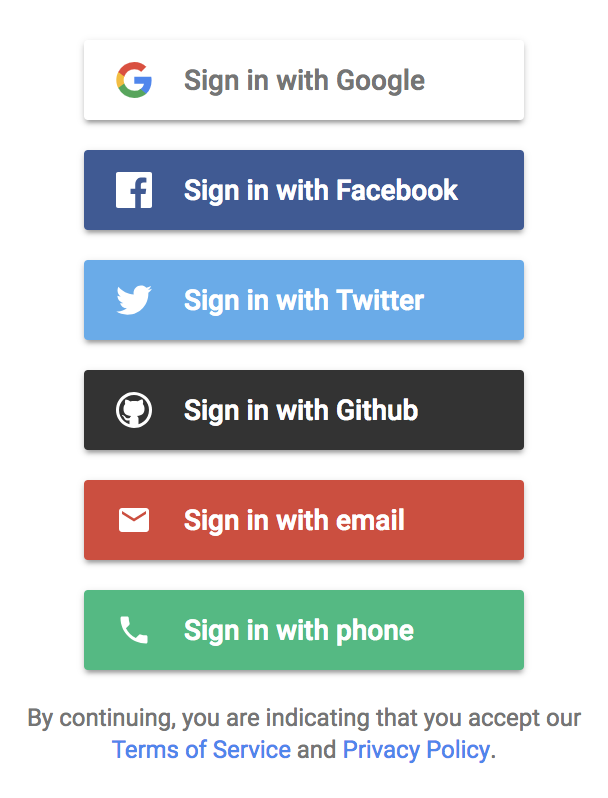
\includegraphics[width=0.6\textwidth, height=11cm]{firebaseui}
	\caption{Inicio de sesión.}\label{fig:firebaseui}
\end{figure}
\FloatBarrier

Como mencionaba arriba, estas funcionalidades que conllevan muy pocas líneas, dotan a nuestra aplicación de seguridad y nos permite tener un control absoluto sobre qué usuarios acceden a ella, como se ve en la figura~\ref{fig:firebase-users}.
\imagen{firebase-users}{Control de usuarios.}



\subsection{Frameworks}
El término \textit{framework}~\cite{wiki:framework} significa entorno o marco de trabajo, y consiste en una estructura conceptual y tecnológica que puede servir de base para el desarrollo software. Incluye programas, bibliotecas y lenguajes interpretados.


En este proyecto se han usado para el desarrollo del mismo los frameworks \nameref{sub:flask}, \nameref{sub:jinja} y \nameref{sub:vue}.


\subsubsection{Flask}\label{sub:flask}
Flask~\footnote{\url{https://flask.palletsprojects.com/en/1.1.x/}} es un \textit{framework} de Python que nos permite crear aplicaciones cliente--servidor de una manera más sencilla, y que no impone ninguna limitación respecto a estructura del proyecto, ni a los componentes que usar durante el desarrollo~\cite{grinberg2014flask}, aunque cabe destacar que en este proyecto se ha seguido la estructura planteada por \textit{Azure} para poder realizar el despliegue.

\subsubsection{Jinja2}\label{sub:jinja}
Para que \textit{Flask} pueda hacer uso de los contenidos \textit{HTML} requiere de la utilización de este motor de plantillas, \textit{Jinja2}~\footnote{\url{https://jinja.palletsprojects.com/en/2.11.x/}}, que consiste en un lenguaje de que permite insertar datos procesados y texto predeterminado en una página \textit{HTML} mediante las etiquetas \verb|{{variable}}| ó \verb||.


\subsubsection{Vue.js}\label{sub:vue}
\textit{Vue}~\footnote{\url{https://vuejs.org/}} es un framework progresivo utilizado para construir interfaces de usuario. Está enfocado únicamente a la capa de visualización, por lo que resulta sencillo integrarlo con otras librerías o incluso en proyectos ya existentes, como es este caso.
Vue ofrece la posibilidad de instalar el cliente mediante \textit{Node.js}\footnote{\url{https://es.vuejs.org/v2/guide/installation.html}}, aunque también permite integrarlo directamente en la capa de visualización incluyendo en los templates del proyecto el \textit{CDN}:

\renewcommand{\lstlistingname}{Vue.js cdn}% Listing -> Algorithm
\renewcommand{\lstlistlistingname}{List of \lstlistingname s}
\begin{lstlisting}[language=html,caption={Versión de desarrollo.}]
<script
src="https://cdn.jsdelivr.net/npm/vue/dist/vue.js"
</script>
\end{lstlisting}
o con
\begin{lstlisting}[language=html,caption={Versión de producción.}]
<script
src="https://cdn.jsdelivr.net/npm/vue"
</script>
\end{lstlisting}
La versión de desarrollo ofrece distintas alertas o advertencias que permiten realizar diferentes trazas a la hora de localizar posibles errores, mientras que la versión de producción está optimizada en cuanto a tamaño y velocidad.
\\
Para poder utilizar \textit{Vue} en nuestros templates, además de incluir el \textit{CDN} debemos crear un componente\footnote{\url{https://vuejs.org/v2/guide/components.html}}, al que le añadiremos una variable. Esto se debe a que realmente la estructura y el nombre de los elementos de Vue es algo diferente a los que ya conocemos de \textit{HTML5}. También es importante tener en cuenta que Vue utiliza los mismos delimitadores que \textit{Flask}: \verb|{{variable}}|. Es por esto por lo que a nuestro componente o variable debemos añadir la línea \verb|delimiters:['[[',']]']| para cambiarlos.


\section{Bibliotecas}
En este apartado se explicarán brevemente las bibliotecas utilizadas para en el desarrollo.

\subsection{JQuery}
\textit{JQuery}~\cite{doc:jquery} es una biblioteca JavaScript que hace que la manipulación de documentos HTML, el manejo de eventos y las peticiones Ajax sean más sencillas de usar y manipular. Además, una de sus ventajas principales es que funciona en prácticamente todos los navegadores web.

\subsection{NetworkX}\label{sub:networkx}
\textit{NetworkX} es la biblioteca por excelencia de Python para trabajar con grafos y redes. Permite crear, manipular y estudiar su estructura.
\\

\noindent Características:
\begin{itemize}
	\item Estructuras de datos para grafos simples, grafos dirigidos y multigrafos.
	\item Contiene la gran parte de algoritmos utilizados para el estudio y modificación de grafos.
	\item Los nodos pueden ser <<cualquier cosa>> como por ejemplo texto, imágenes o números.
	\item Los arcos pueden tener diferentes atributos o datos, como el peso, distancia...
	\item Es de código abierto.
\end{itemize}


\subsection{Tube Map - D3}
Esta biblioteca permite dibujar mapas muy similares a los mapas que hoy podemos ver en el metro, con sus estaciones, paradas e intersecciones~\cite{doc:tubemap}.
\\
Se intentó implementar en el proyecto durante dos Sprints, pero se llegó a la conclusión que no se podía generar la estructura necesaria en el archivo JSON para el dibujado del mapa. Esta estructura debía contener coordenadas con números enteros y estar ordenadas de tal forma que se indicasen las esquinas y cruces que debía haber entre las diferentes líneas, o en este caso, recorridos.

\subsection{SVGWRITE}\label{sub:svgwrite}
\textit{SVGWRITE}~\cite{doc:svgwritedocs}, como su propio nombre sugiere, sirve para la creación y dibujado de gráficos vectoriales escalables. Su principal inconveniente es que no permite leer o modificar un archivo ya existente, es decir, sólo permite su creación desde cero.

\subsection{Snap.svg}\label{sub:snap}
\textit{Snap.svg}~\cite{doc:snapsvg} es una biblioteca JavaScript que permite crear gráficos vectoriales interactivos y fácilmente manipulables en el lado del cliente. Su uso es similar al uso de jQuery.


\subsection{\LaTeX}
Como herramienta para realizar la documentación se ha escogido \LaTeX{}~\cite{wiki:latex}, lenguaje orientado a la creación de documentos que presenten una alta calidad tipográfica.

\subsubsection{MiK\TeX}
\textit{MiK\TeX} es una distribución libre de \LaTeX{} que incluye tipografías compiladores y herramientas para generar bibliografías e índices.


\section{Despliegue}
La idea de plantear el proyecto como una aplicación web sugiere que ésta tiene que ser fácilmente accesible por lo usuarios, cosa que no es cierta si para poder usarla tienen que descargarse el código, configurar el proyecto y ejecutarlo en su propio dispositivo. Por esta razón, valoré desplegar la aplicación en Azure\footnote{\url{https://azure.microsoft.com}}.

Elegí esta plataforma por que con el correo de la Universidad podemos tener acceso a un plan de estudiantes, llamado \textit{Azure for Students}\footnote{\url{https://azure.microsoft.com/es-es/free/students/}}, que permite, además de acceso a diversos tutoriales sobre computación en la nube, desplegar nuestra aplicación de manera gratuita, aunque por supuesto también tiene varios planes de pago.


Link de la aplicación: \url{http://tfgmetrominuto.azurewebsites.net/}.